\subsubsection{От чего зависит проводимость п/п и каким образом ею можно управлять?}

К полупроводникам относят вещества, которые при комнатной температуре имеют удельное электрическое сопротивление $\rho$ в пределах от $10^{-3}\div 10^{-2} - 10^8\div 10^9$ Ом$\times$см.

Сопротивление чистых полупроводников сильно зависит от температуры, причём с ростом температуры оно уменьшается. Так, для полупроводников температурный коэффициент может достигать значений $5-6\%$ на $1^{\circ}$C.

В транзисторах чаще всего используются кремний и германий. Однако закономерности, характерные для этих материалов, распространяются на весь класс полупроводников.

Германий и кремний являются IV-валентными элементами и имеют \textbf{тетраэдрический} тип решётки, или решётку типа \textbf{алмаза}, для которой характерно одинаковое расстояние центрального атома от четырёх угловых. Каждый угловой в свою очередь является центровым для четырёх других ближайших атомов. Совокупность тетраэдров образует элементарную ячейку.

Удобно пользоваться плоским эквивалентом тетраэдрической структуры, в котором сохранена главная особенность решетки типа алмаза(равенство расстояний).

\begin{center}
	\begin{figure}[h!]
		\center{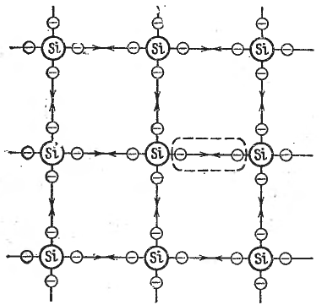
\includegraphics[scale=0.7]{2D.png}}
		\caption{"Плоский" эквивалент тетраэдрической решётки}	
		\label{2D}
	\end{figure}
\end{center}

Такая совершенно однородная структура, представленная на Рис. \ref{2D}, характерна лишь для кристалла, который имеет температуру абсолютного нуля. По мере нагревания часть валентных связей нарушается.

Нарушение валентных связей приводит к одновременному образованию свободных элементов и пустых мест, - к т.н. генерации пар электрон-дырка. Дырка ведёт себя подобно частице с элементарным положительным зарядом.

Таким образом, в полупроводниках имееются два типа подвижных носителей заряда - электроны и дырки, причём при нагревании чистого и однородного полупроводника(называемого \textbf{собственным}), свободные электроны и дырки всегда образуются парами.

Проводимость, обусловленную наличием примесных атомов, нарушающий структуру кристаллической решетки, называют \textbf{примесной} или \textbf{дефектной}.

\begin{itemize}
\item Электронная проводимость или проводимость n-типа

Если ввести в n-валентный полупроводник (n+1)-валентную примесь, то n из ее валентных электронов образуют устойчивую связь. Один электрон оказывается слабо связанным с ядром и достаточно легко отрывается от него и делается свободным. При этом примесный атом превращается в неподвижный ион с единичным положительным зарядом. Тк неподвижен $\Rightarrow$ не может участвовать в проводимости. Свободные электроны примесного происхождения добавляются к собственным свободным электронам, порожденным термогенерацией $\Rightarrow$ проводимость полупроводника делается преимущественно электронной. Такие проводники называются проводниками n-типа. Примеси, обусловливающие электронную проводимость, называются \textbf{донорными}.

\item Дырочная проводимость или проводимость p-типа

Если ввести в n-валентный полупроводник (n-1)-валентную примесь, то (n-1) ее электронов образуют валентную связь. Однако для образования устойчивой связи требуется дополнительный электрон. Этот электрон отбирается из основной решётки и превращает атом бора в неподвижный отрицательный ион. На том месте, откуда пришёл электрон, образуется дырка, которая добавляется к собственным дыркам, порожденным термогенерацией. Такие проводники называются проводниками p-типа. Примеси называются \textbf{акцепторными}. 
\end{itemize}

Отрыв "лишнего"  электрона от донора и "недостающего" электрона для акцептора требует затраты некоторой энергии(энергия ионизации или активации примеси). 

Т.к. в п/п один тип подвижных носителей заряда превалирует над другим, принято называть те носители, которые составляют большинство, основными. Меньшинство - неосновными.
